\documentclass[12pt,a4paper]{article}

\usepackage[T1]{fontenc}
\usepackage[english]{babel}
\usepackage[utf8]{inputenc}
\usepackage{lmodern}
\selectlanguage{english}
\usepackage{graphicx}
\usepackage{biblatex}
\usepackage{csquotes}
\addbibresource{bib.bib}

\begin{document}


\nocite{*}

\pagenumbering{gobble}
\clearpage
\begin{figure}[h]
\centering

\includegraphics[scale=0.4]{media/politechnika_sl_logo_pion_en_rgb.jpg}
\end{figure}
\hspace{3cm}
\begin{center}Project documentation \end{center}
\begin{center}2021/2022\end{center}
\hspace{3cm}
\begin{center}\large\textbf{Advances of neural networks computing}\end{center}
\hspace{7cm}
\begin{flushright}Faculty: Informatics
\end{flushright}
\begin{flushright}Team members:
\par
\textit{Dawid Bitner}
\par
\textit{Daniel Broczkowski}
\par
\textit{Damian Kwaśniok}
\end{flushright}
\vfill
\begin{center}Gliwice, 2021/2022\end{center}

\newpage
\pagenumbering{arabic}
\renewcommand*\contentsname{Table of content}
\tableofcontents

\newpage
\section{Introduction}

\subsection{Purpose of the project}
The aim of the project was to create a system based on human-computer interaction. The design team decided to implement an application that recognizes whether the person standing in front of the camera has a face mask on. The project is called "face mask detector". The main goal of the project was to create a useful application that could be used in the area of public space (universities, offices, other public institutions) and that could be used by private entities - the project was to show how human-computer interaction can be used in everyday life.

\subsection{Project team}
Dawid Bitner    :: Developer\newline
Daniel Broczkowski    ::Developer\newline
Damian Kwaśniok    :: Developer\newline

\newpage

\section{Design assumptions}
The main design dependencies determined by the solution implementation team include: 
\begin{itemize}
\item universality
\item scalability
\item the possibility of improvement
\item use \textit{Machine Learning}
\item based on human-computer interaction 
\end{itemize}

According to the team responsible for the project, all assumptions have been met. The face mask detection system can be run on devices with different operating systems, e.g. \textit{Microsoft Windows}, \textit{Linux}. The project can be run on any environment where\textit{Python 3} interpreter with libraries has been installed.

The program is scalable and susceptible to improvement, it can be constantly improved by adding additional options in the future, e.g. in addition to recognizing the mask on the face, adding recognition of a person in front of the camera. It is especially useful if, in addition to verifying the wearing of a mask, you also need to verify the person in front of the camera, e.g. if he or she is an academic teacher, employee, etc.

The program has been trained to detect a mask on the face using machine learning. There is also human-computer or human-machine interaction. The person approaches the camera, the software verifies whether he or she has a mask on, then, based on the result of the algorithm's operation, a decision can be made as to the result. 
\newpage

\section{Implementation}
The project was implemented based on the \textit{Python} programming language. components of such libraries as \textit{TensorFlow}, \textit{Keras}, \textit{Numpy} were used. 

First, the data set for overtraining was selected. It should be emphasized that the selected set is not perfect, only light-colored surgical masks were used in it, and in some cases they were glued to the photo by means of graphic processing. For this reason, as will be presented in the next chapter, the system does not fully recognize the situation in which the person in front of the camera is wearing a dark mask. Photos for training and testing have been divided into two groups: with and without a mask. 
\begin{figure}[h!]
    \centering
    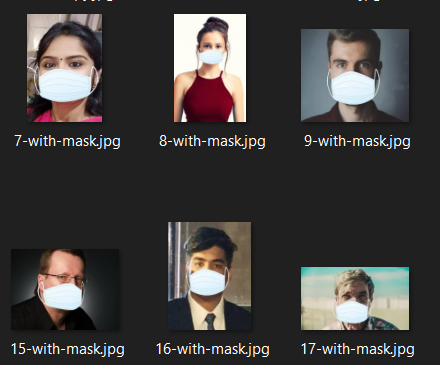
\includegraphics[scale = 1]{media/mask.png}
    \caption{Part of the dataset for training - with mask }
    \label{fig:Rysunek1}
\end{figure}
\newpage
Then a script with an 8-layer neural network was created, which trains and tests the program.
\begin{figure}[h!]
    \centering
    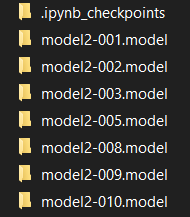
\includegraphics[scale = 1]{media/modele.png}
    \caption{Result models}
    \label{fig:Rysunek1}
\end{figure}
Lastly, a script was written to integrate the camera in the device with the face detection system. The results of the operation are visible in the next chapter.

\section{Research}
During the implementation of the project, the design team was guided by the latest trends in the field of \textit{Machine Learining}, the created network works correctly, does not burden the operating system too much, and, in our opinion, it works quite quickly on the selected data set. In theory, the sytsem should primarily detect a person's head using the face classifier \textit{haarcascade\_frontalface\_default} - which in the \textit{.xml} file contains a set of coordinates developed by the \textit{Intel} company under the \textit{Open Source license} - what it says in the comment in the file. Additionally, the system checks whether the test subject has a mask on or not. In practice, this task is not always fulfilled in one hundred percent, which is shown in the examples below. 

\begin{figure}[h!]
    \centering
    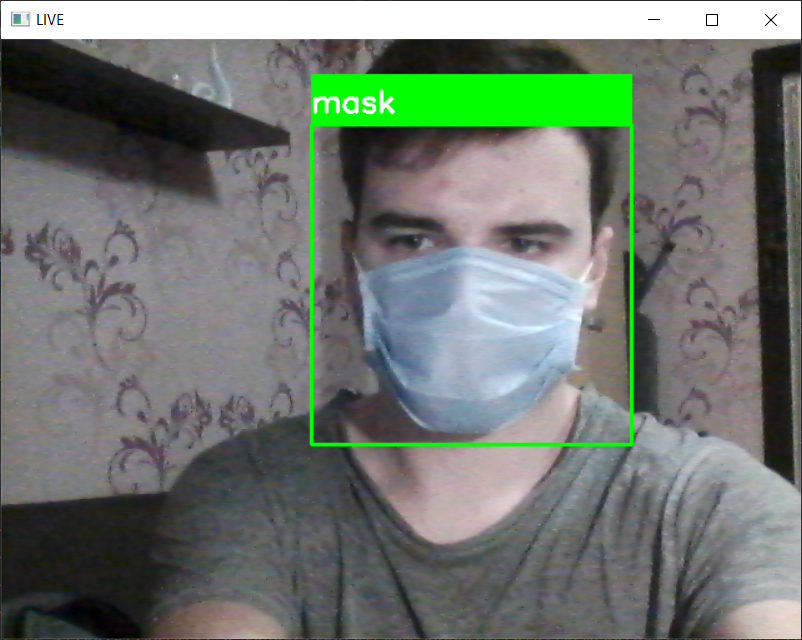
\includegraphics[scale = 0.38]{media/true_z.png}
    \caption{Correctly detected face with a mask.}
    \label{fig:Rysunek1}
\end{figure}

\begin{figure}[h!]
    \centering
    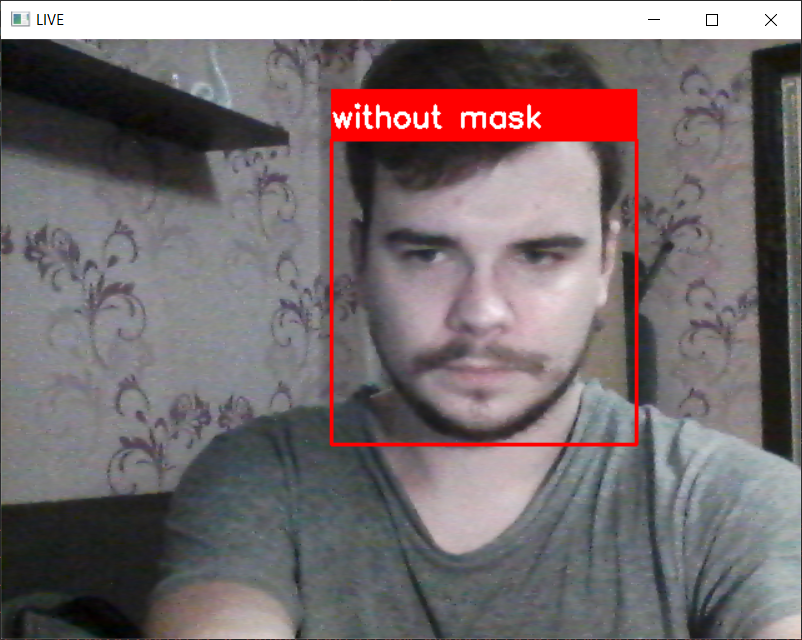
\includegraphics[scale = 0.38]{media/false_bez.png}
    \caption{Correctly detected face without mask}
    \label{fig:Rysunek2}
\end{figure}
\newpage
The first two cases were correctly identified. This is mainly due to two factors. The first is good lighting - the examined face is bright and its contours contrast with the background. The second factor is the training set itself, which is not of the quality that the design team would like. Often, masks were attached to photos in graphic programs, which means that the photo scene is not normalized and the mask clearly contrasts with the rest of the head (it is worth noting that in the discussed case, blue-colored masks were used).

\newpage

\section{Summary and Conclusions}

\begin{itemize}
\item \textit{Summary}

The system is highly effective. Taking into account the test and training sets, it amounts to approx. \textit{92\%} taking into account the requirement of the light mask test. In our opinion, it works very well for the dataset it has been trained on. The system also correctly detects the existence of a face. 

\item \textit{Conclusions}

The system is simple, easy to run on various environments, in our opinion, this is what modern software should strive for. The system incorrectly detects dark masks, the next iteration of the system training should run on slightly more differentiated test images (different colored masks). This is certainly the most important area to be worked on in this implementation.  

\end{itemize}

\end{document}
